\documentclass[../report.tex]{subfiles}
\begin{document}	

\chapter{Design and simulation}
\gls{tpr} can be achieved in different ways, discussed in section \ref*{sec:active_pr}. In this thesis, the goal is to achieve \gls{tpr} using MEMS for a broadband spectrum including C and L bands. Moreover, the idea is to optimize the design to achieve high \gls{per} and low \gls{il}.  
	
	\section{Approach}
	\gls{mems} \gls{tpr} can be approached in 2 ways. In a first approach, initially a passive \gls{pr} can be designed by introducing asymmetry and another MEMS tunable waveguide is introduced which impedes polarization rotation by reintroducing symmetry in the effective waveguide. In a second approach, the technique is reversed i.e. the MEMS tunable waveguide is used to introduce asymmetry in the waveguide structure which rotates polarization. Without the MEMS structure the polarization is not rotated. In the design principle of the \gls{tpr} described here, the first approach is being followed.  
	
	\section{Designing the experiment}
	To design the geometry of the waveguide standard mode solver softwares are used. Both, Comsol\cite{comsol_2015} and CST \cite{cst_2015} are used to solve the modes in equation \ref{eq:helmholtz_eq_wg_general}. Mostly, in this thesis Comsol is used to find and optimize the port modes in 2-D geometry. Whereas, CST is used to optimize the 3-D structure by studying the transmission parameters (S-parameters).
	
	% obtained for output port mode after running the simulation. Air cladding is considered around the Silicon base waveguide for setting up the simulation.
		
		\subsection{Design principle}
To design a \gls{pr} in nanometer scale, precision is a key factor. Index profile of chosen silicon can also affect the structural dimensions of the design in a rigorous manner. Meshing of the geometry, cladding dimensions and its material composition, frequency domain of the solvers etc. are the key things to watch for in designing the simulation in the mode solver softwares. As the idea is to make the \gls{tpr} as broadband as possible, it is necessary to do frequency analysis simulation for a wide-band spectrum in which the optical fibers for telecommunications work. As the operating wavelength of the telecommunications optical fiber network in C-band and L-band are between $\SI{1530}{\nano\metre}$ and $\SI{1625}{\nano\metre}$, the corresponding frequency domain becomes $\SI{184.48}{\THz}$ - $\SI{195.94}{\THz}$.
	
		\subsection{Design A: Single stair Si waveguide on SOI with air cladding based on mode hybridization}
Initially, a single stair waveguide is being designed for \gls{pr}. To find out the dimensions for obtaining $45{^\circ}$ hybridized modes, Comsol 2D mode solver is used. 

\subsubsection{Waveguide geometry}
Throughout the next sections the dimensions of the stair waveguide are defined in terms of rib, slab and base described in Fig. \ref{fig:3_wg_structure}.   

\begin{figure}[H] %h
	\centering
	\includegraphics[width=0.75\textwidth]{3-wg-structure}
	\caption{Stair waveguide geometry}
	\label{fig:3_wg_structure}
\end{figure}


\subsubsection{Optimized dimensions of primary PR waveguide}
At $45{^\circ}$, the components of the E-fields in the hybridized modes must be such that, $E_X \approx E_Y$. Hence, $\dfrac {Avg(E_{X_{mode}})} {Avg(E_{Y_{mode}})} \rightarrow 1$. As a result, 

\begin{equation}\label{eq:wg_dim_eq}
\sum _{mode}Real\left| \log _{10}\dfrac {Avg(E_{X_{mode}})} {Avg(E_{Y_{mode}})}\right| \rightarrow 0. 
\end{equation}

\begin{figure}[H] %h
	\centering
	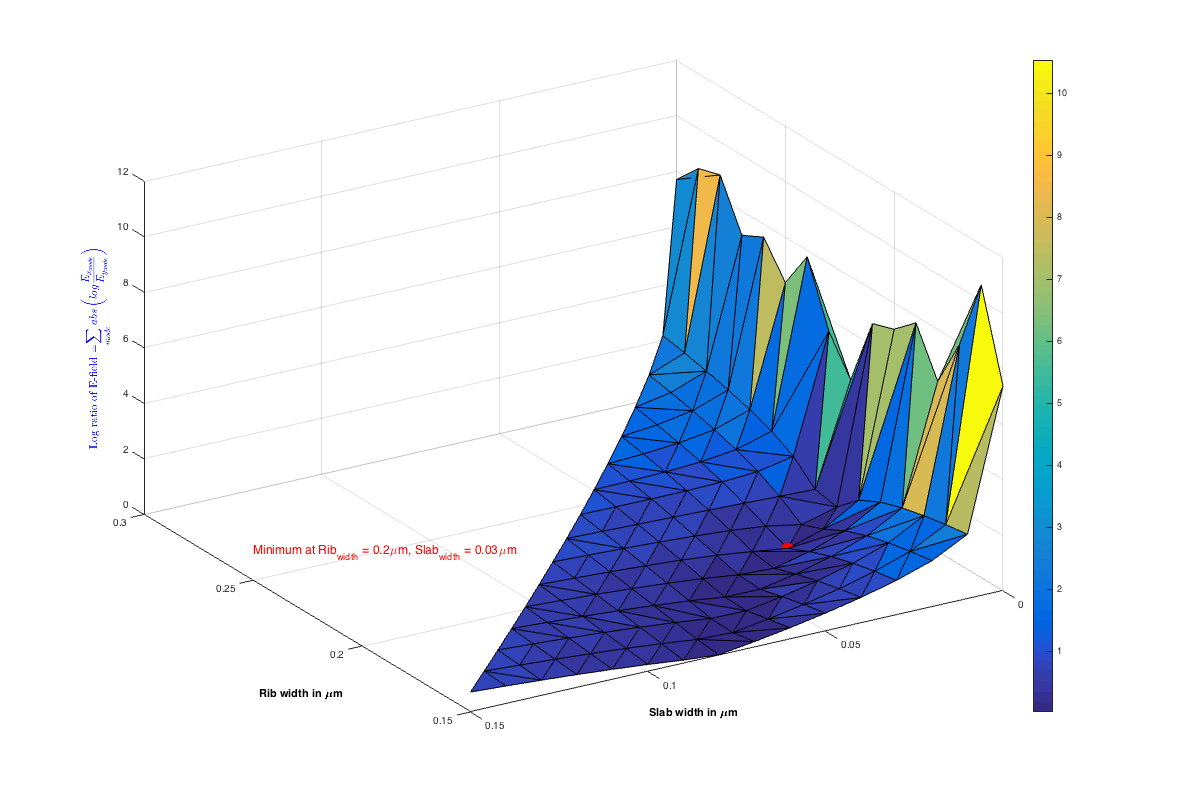
\includegraphics[width=1\textwidth]{3-graph-mode-sum}
	\caption{Summation of real part of absolute value of the logarithmic ratio of $E_x$ and $E_y$ fields plotted against rib and base width in an area chart using MATLAB}
	\label{fig:3_graph_mode_sum}
\end{figure}  
\noindent Hence, the minimum point on the graph represents the best dimensions on the waveguide for obtaining the hybridized modes at $45{^\circ}$. In this case the best dimensions were obtained at $\chem{Base_{width}}$ = 230nm and $\chem{Rib_{width}}$ = 200nm. The total height of the waveguide is 220nm and the$Slab_{height}$ = 110nm. It can visualized that in the modes in Fig. \ref{fig:3_mode1_200_230} and Fig. \ref{fig:3_mode2_200_230}, that the effective modes are hybridized at $45{^\circ}$ for the first 2 hybrid modes obtained using Comsol simulation. It is necessary to double check the E-fields orientation to make sure that only the correct modes are chosen because in simulation a larger cross-section than the waveguide cross-section is excited. This excitation might produces modes for which the equation \ref{eq:wg_dim_eq} satisfies but the modes are not hybridized at $45{^\circ}$. Lastly, the height in the geometry is chosen around 110nm for the current limitation of the dry-etch step in the fabrication process present in the lab. A double stair waveguide could also have been chosen, but that would increase the fabrication steps.
\begin{figure}[H] %h
	\begin{subfigure}[t]{0.45\textwidth}
		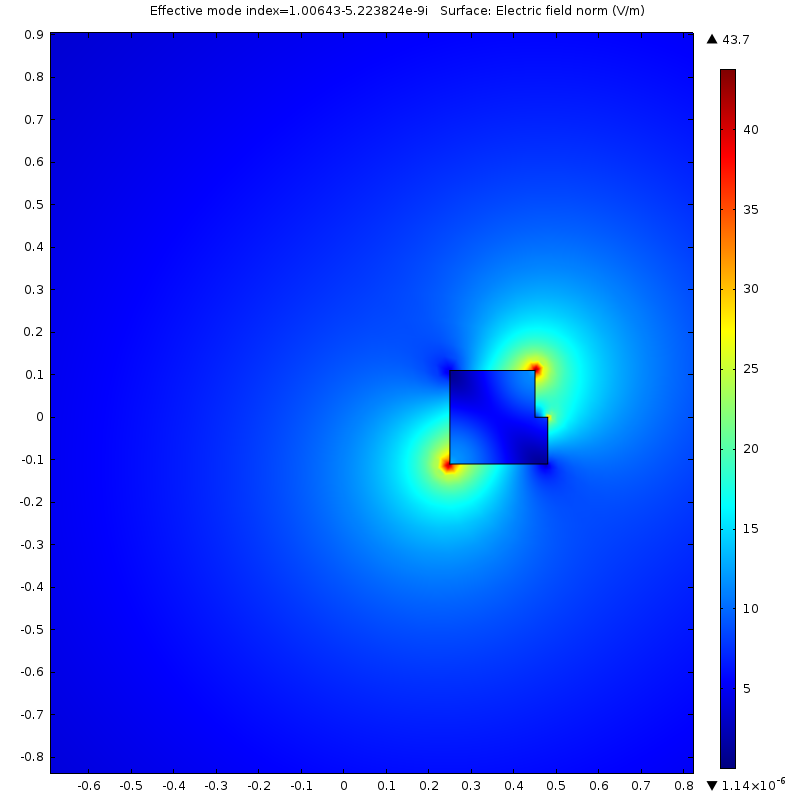
\includegraphics[width=\textwidth]{3-mode1-200-230}
		\caption{$1^{st}$ hybrid mode in the cross-section}
		\label{fig:3_mode1_200_230}
	\end{subfigure}
	\hfill
	\begin{subfigure}[t]{0.45\textwidth}
		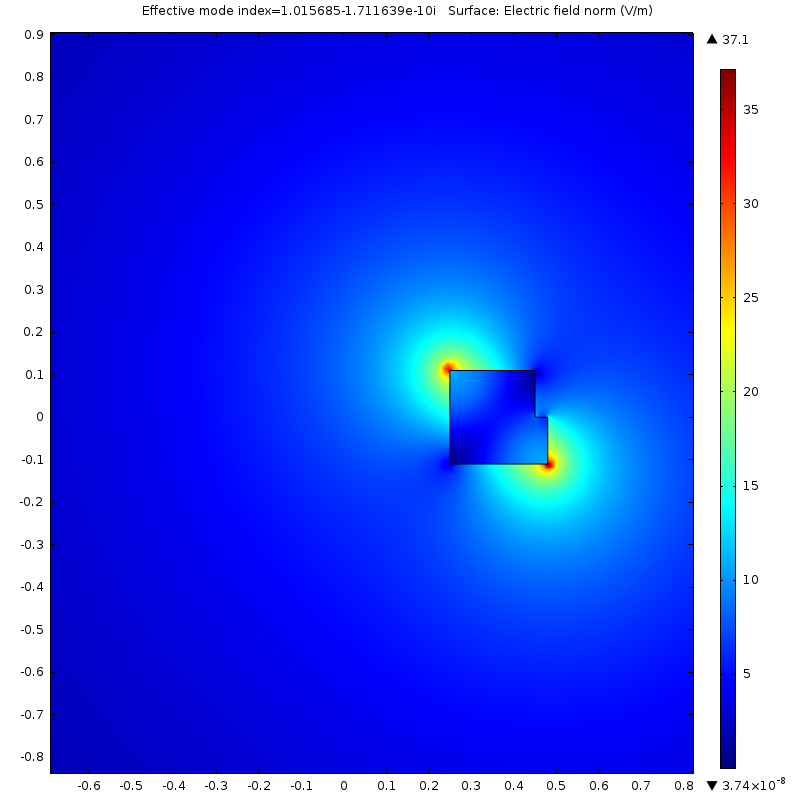
\includegraphics[width=\textwidth]{3-mode2-200-230}
		\caption{$2^{nd}$ hybrid mode in the cross-section}
		\label{fig:3_mode2_200_230}
	\end{subfigure}
	\caption{Fundamental hybrid modes in the cross-section with $\chem{Rib_{width}}$ = 200nm, $\chem{Rib_{height}}$ = 110nm, $\chem{Base_{width}}$ = 230nm, $\chem{Slab_{height}}$ = 110nm, obtained using Comsol 2-D eigenmode simulation}
\end{figure}

\begin{figure}[H] %h
	\begin{subfigure}[t]{0.45\textwidth}
		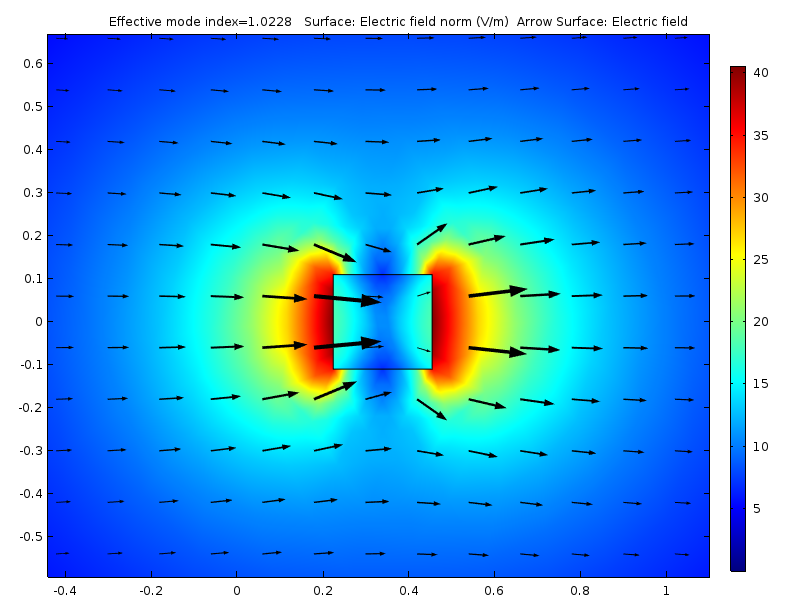
\includegraphics[width=\textwidth]{3-mode1-230-230}
		\caption{\gls{te} mode in the cross-section}
		\label{fig:3_mode1_230_230}
	\end{subfigure}
	\hfill
	\begin{subfigure}[t]{0.45\textwidth}
		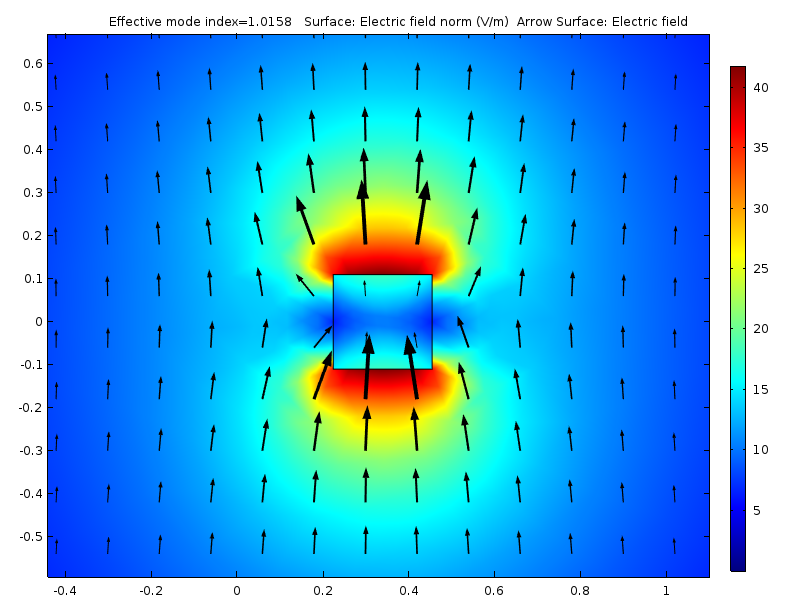
\includegraphics[width=\textwidth]{3-mode2-230-230}
		\caption{\gls{tm} mode in the cross-section}
		\label{fig:3_mode2_230_230}
	\end{subfigure}
	\caption{Fundamental modes in the cross-section with Width = 230nm, Height = 220nm, obtained using Comsol 2-D eigenmode simulation}
\end{figure}

\noindent Also, since the port dimensions are different from the cross-section dimensions it is necessary to check if the 2 fundamental modes can be supported by the ports. Hence, port mode simulation for the first two fundamental modes in waveguide with dimensions 230$\times$220 nm are calculated and the results obtained are displayed in Fig. \ref{fig:3_mode1_230_230} and Fig. \ref{fig:3_mode2_230_230}. This corroborates that the 2 fundamental modes \gls{te} and \gls{tm} are supported in the ports.\\

\noindent Next, the effective \gls{ri} for both the port modes are obtained using CST by doing a parametric sweep over the operating frequencies of C and L-band. The results are displayed in Fig. \ref{fig:3_effective_ri_200_230}. 

\begin{figure}[H] %h
	\centering
	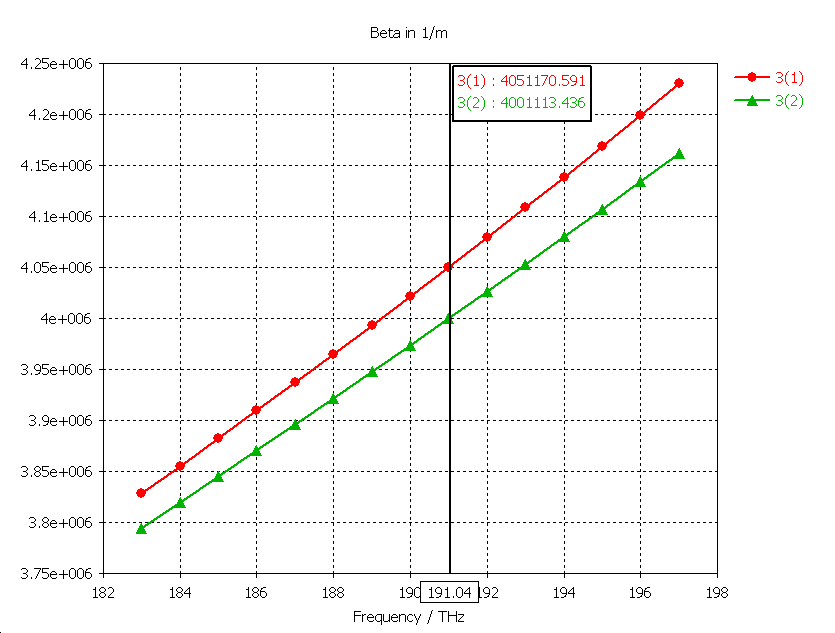
\includegraphics[width=0.9\textwidth]{3-effective-ri-200-230}
	\caption{Simulated effective \gls{ri} profile for the port modes in the cross-section of $\chem{Rib_{width}}$ = 200nm, $\chem{Rib_{height}}$ = 110nm, $\chem{Base_{width}}$ = 230nm, $\chem{Slab_{height}}$ = 110nm, obtained using CST 3-D simulation}
	\label{fig:3_effective_ri_200_230}
\end{figure}

\noindent The required length of the cross-section is obtained using \ref{eq:jones_matrix_wp1}. Since, $\beta_1$ = $4.051 \times 10^6$  and $\beta_2$ = $4.001 \times 10^6$. Hence, $L = \dfrac{\pi}{\beta_1 - \beta_2} \approx 51nm$. This means the length of the stair cross-section would be around 51nm. Effective \gls{ri} is dependent on frequency and so the cross-section length is also dependent on the frequency. The length is calculated at around $\SI{191}{\THz}$, so that the whole of the band ($\SI{184.48}{\THz}$ - $\SI{195.94}{\THz}$) can be covered for a relative good performance. This results could have also been obtained from COMSOL from the effective \gls{ri} calculation as shown in \ref{eq:lpi_calc}.

\begin{equation}\label{eq:lpi_calc}
L_\pi =  \dfrac {\pi} {\beta_1 - \beta_2} = \dfrac {\pi} {\dfrac {2\pi} {\lambda}\left(n_1 - n_2\right)} = \dfrac {\lambda} {2(n_1 - n_2)}
\end{equation}

\begin{figure}[H] %h
	\centering
	\includegraphics[width=0.9\textwidth]{3-wg-design-1}
	\caption{Design of single-stair waveguide with initial dimensions at the port as width = 230nm and height = 220 nm. Stair cross-section dimensions are: $\chem{Rib_{width}}$ = 200nm, $\chem{Rib_{height}}$ = 110nm, $\chem{Base_{width}}$ = 230nm, $\chem{Slab_{height}}$ = 110nm, and cross-section length = \SI{51}{\micro\meter}. The output port is along the Z-axis, shown in the figure}
	\label{fig:3_wg_design_1}
\end{figure}

\noindent The 3D-design is simulated in CST with air cladding and with the previously estimated dimensions. The input and output ports are defined on the waveguide, which supports the two fundamental modes. As shown in Fig. \ref{fig:3_wg_design_1}, the stair cross-section can be envisaged if a Z-plane is cut in the asymmetric part of the waveguide.\\

\noindent Next, the S-parameters of the design are verified. The S-parameter is being labelled as follows,
\begin{equation}\label{eq:s_parameter_label}
SA(M),SB(N),
\end{equation}
where A=output port, B=input port and M,N = mode number. For example, S2(2),S1(1) means that input port is 1 and the mode is 1 whereas, output port is 2 and the mode at the output port is 2. Hence, S2(1),S1(2) and S2(2),S1(1) needs to be checked along with S2(1),S1(1) and S2(2),S1(2) for calculating the \gls{per}. The S-parameters obtained from the simulation shown in Fig. \ref{fig:3_stair_s_param_200_230} (for, 200nm$\times$230nm) verifies that the model works according to the design principle with good \gls{per} over the whole band. 

%For example, the $PER_{191 THz} = 10 log_{10} $

\begin{figure}[H] %h
	\centering
	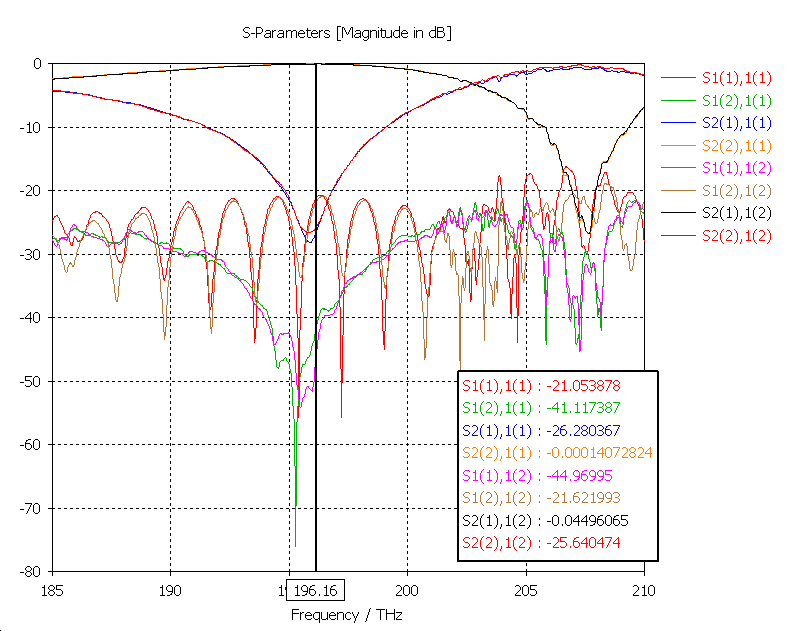
\includegraphics[width=0.9\textwidth]{3-stair-s-param-200-230}
	\caption{Simulated S-parameters in the single-stair waveguide with initial dimensions at the port as width = 230nm and height = 220 nm. Stair cross-section dimensions are: $\chem{Rib_{width}}$ = 200nm,$\chem{Rib_{height}}$ = 110nm, $\chem{Base_{width}}$ = 230nm, $\chem{Slab_{height}}$ = 110nm, and cross-section length = \SI{51}{\micro\meter} obtained using CST 3-D simulation}
	\label{fig:3_stair_s_param_200_230}
\end{figure}

\begin{figure}[H] %h
	\centering
	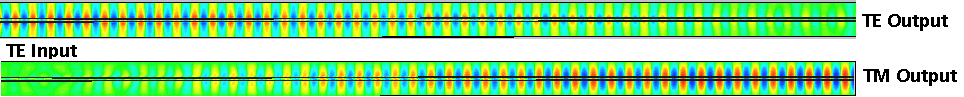
\includegraphics[width=\textwidth]{3-te-tm}
	\caption{\gls{te} to \gls{tm} mode conversion view from top perspective}
	\label{fig:3_te_tm}
\end{figure}

\begin{figure}[H] %h
	\centering
	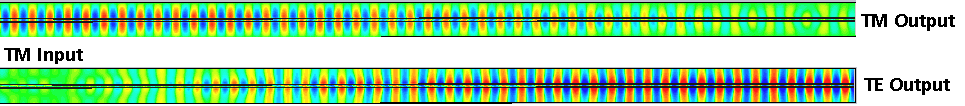
\includegraphics[width=\textwidth]{3-tm-te}
	\caption{\gls{tm} to \gls{te} mode conversion view from top perspective}
	\label{fig:3_tm_te}
\end{figure}

\subsubsection{Optimized dimensions of secondary MEMS waveguide}
After finding the dimensions of the passive \gls{pr}, the design of the \gls{mems} tunable waveguide was designed to neglect the effect of rotation. Intuitively, if any waveguide which is the mirror image of the bus waveguide is place along side the bus waveguide, then \gls{pr} effect would be nullified. This is verified by plotting the graph in Fig. \ref{fig:3_graph_mode_sum_mems}. Since, at TE or TM mode, $E_X \gg E_Y$, or $E_Y \gg E_X$. Hence, $\left|\dfrac {Avg(E_{X_{mode}})} {Avg(E_{Y_{mode}})}\right| \rightarrow \infty$, or $\left|\dfrac {Avg(E_{Y_{mode}})} {Avg(E_{X_{mode}})}\right| \rightarrow \infty$, depending on \gls{te} or \gls{tm}-mode.
Hence, 
\begin{equation}\label{eq:mems_dim_eq}
\sum _{mode}Real\left| \log _{10}\dfrac {Avg(E_{X_{mode}})} {Avg(E_{Y_{mode}})}\right| \rightarrow \infty,
\end{equation}
and the maximum points on the graph will represent the dimensions of the \gls{mems} structure for which, there is no \gls{pr}. Logarithmic scale is used to plot the data in a manageable way. The supermodes are also verified in the cross-section in Fig. \ref{fig:3_mems_mode1_200_230} and Fig. \ref{fig:3_mems_mode2_200_230} to make sure higher order modes are not supported.

\begin{figure}[H] %h
	\centering
	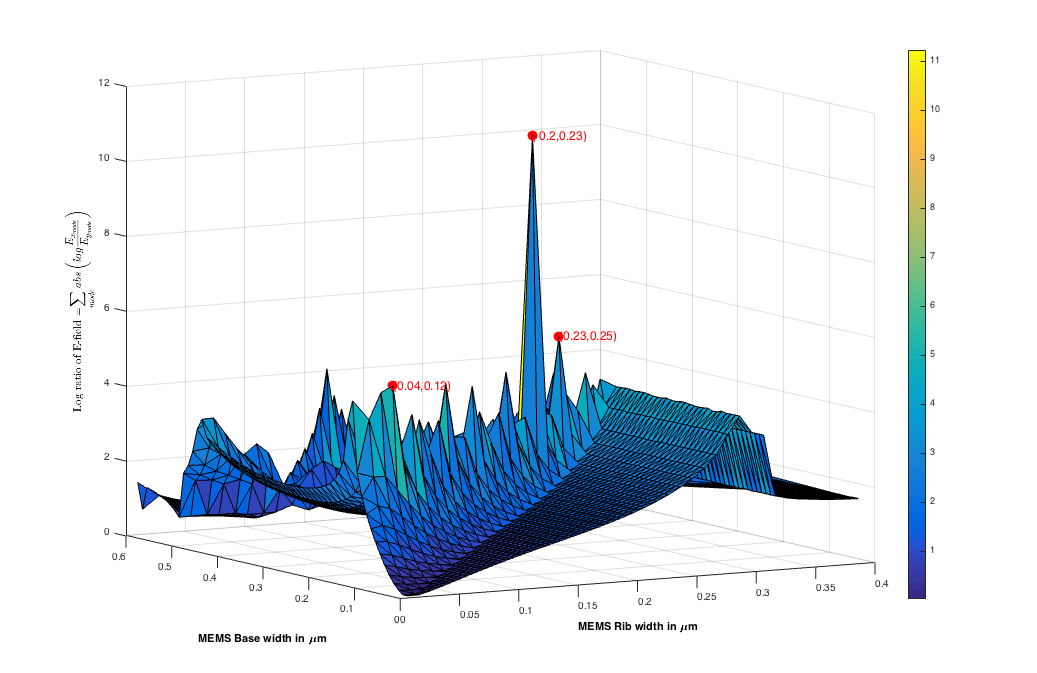
\includegraphics[width=1\textwidth]{3-graph-mode-sum-mems}
	\caption{Summation of real part of absolute value of the logarithmic ratio of $E_x$ and $E_y$ fields plotted against rib and total width in an area chart using MATLAB}
	\label{fig:3_graph_mode_sum_mems}
\end{figure}
		
\begin{figure}[H] %h
	\begin{subfigure}[t]{0.45\textwidth}
		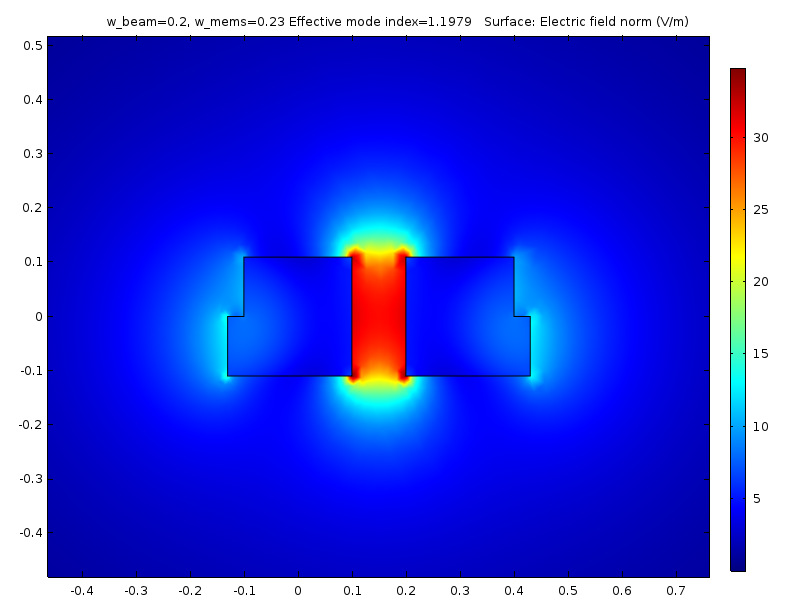
\includegraphics[width=\textwidth]{3-mems-mode1-200-230}
		\caption{\gls{te} mode with the \gls{mems} cross-section}
		\label{fig:3_mems_mode1_200_230}
	\end{subfigure}
	\hfill
	\begin{subfigure}[t]{0.45\textwidth}
		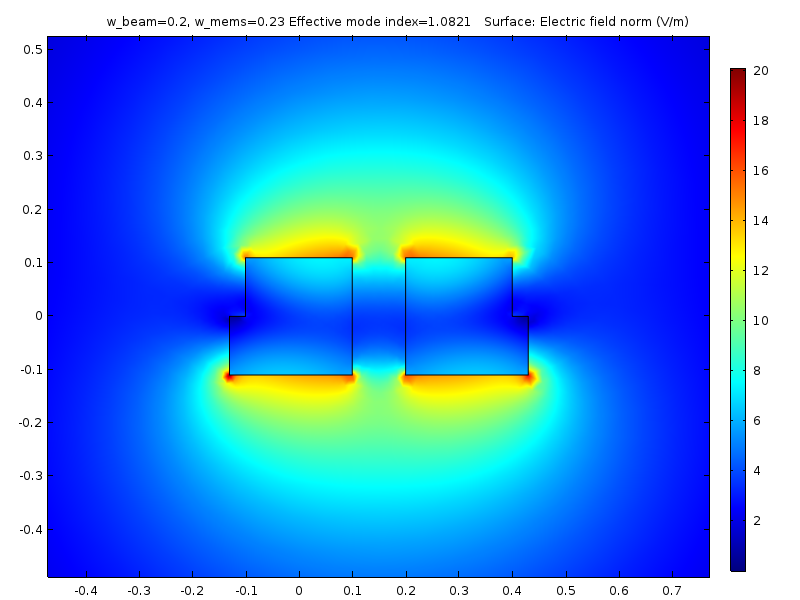
\includegraphics[width=\textwidth]{3-mems-mode2-200-230}
		\caption{\gls{tm} mode with the MEMS cross-section}
		\label{fig:3_mems_mode2_200_230}
	\end{subfigure}
	\caption{Modes in the cross-section with $\chem{Rib_{width}}$ = 200nm, $\chem{Slab_{width}}$ = 30nm, $\chem{Slab_{height}}$ = $\chem{Rib_{height}}$ = 110nm, in both bus and \gls{mems} waveguide, obtained using Comsol 2-D simulation}
\end{figure}

In this case the best dimensions for the \gls{mems} waveguide comes out as, $\chem{Rib_{width}}$ = \SI{200}{nano meter}, $\chem{Rib_{height}}$ = \SI{110}{nano meter}, $\chem{Base_{width}}$ = \SI{230}{nano meter}, $\chem{Slab_{height}}$ = \SI{110}{nano meter}. Fig. \ref{fig:3_mems_mode1_200_230} and Fig. \ref{fig:3_mems_mode2_200_230}, obtained using Comsol 2D simulation displays the port modes in the cross-section. This corroborates the claim that the \gls{mems} waveguide must be mirror image of the bus waveguide to inhibit \gls{pr}.

\subsubsection{Device tolerance}
When fabricating devices in nanometer scale often it is very difficult to control the device dimensions precisely. Hence, a brief study on simulation level is performed to check for deviance resulting due to variations in etch depth during the fabrication process discussed later in section \ref{sec:fab_process}.\\  

Since the wafer used in the fabrication process is of height 220nm, the different etch depths considered are 100nm and 130nm which corresponds to 120nm and 90nm slab height respectively. Fist 20 minimum values of $\sum _{mode}Real\left| \log _{10}\dfrac {E_{X_{mode}}} {E_{Y_{mode}}}\right|$, is plotted against $\chem{Rib_{width}}$ and $\chem{Slab_{width}}$ in the following figure in Fig. \ref{fig:3_graph_mode_sum_120nm_slab_height} for an etch depth of 100nm. 

\begin{figure}[H] %h
	\centering
	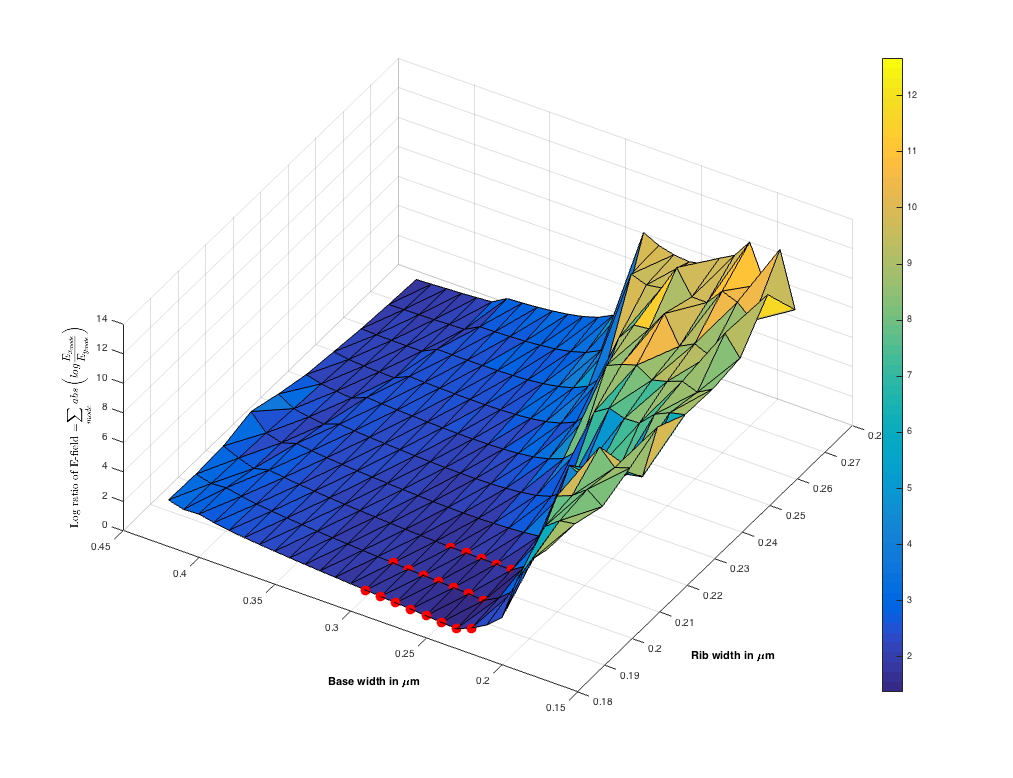
\includegraphics[width=1\textwidth]{3-graph-mode-sum-120nm-slab-height}
	\caption{20 least values, representing the summation of real part of absolute value of the logarithmic ratio of $E_x$ and $E_y$ fields, plotted against rib and total width in an area chart using MATLAB for $\chem{Slab_{height}}$ = 120nm}
	\label{fig:3_graph_mode_sum_120nm_slab_height}
\end{figure}
\noindent It can be seen in the above Fig. \ref{fig:3_graph_mode_sum_120nm_slab_height} that the hybridized modes appear to be at $45^{\circ}$ around $\chem{230nm \leq Base_{width} \leq 300nm}$ and $\chem{180nm \leq Rib_{width} \leq 200nm}$. So, if the $\chem{Rib_{width}}$ and $\chem{Base_{width}}$ are controlled in the fabrication process, the device can still function and needs to be characterized accordingly.\\

The same process is followed for a speculated etch depth of 130nm and the 20 best dimensions are plotted which comes out to be $\chem{230nm \leq Base_{width} \leq 300nm}$ and $\chem{160nm \leq Rib_{width} \leq 200nm}$. The exact pairs can be identified in the Fig. \ref{fig:3_graph_mode_sum_90nm_slab_height}.
\begin{figure}[H] %h
	\centering
	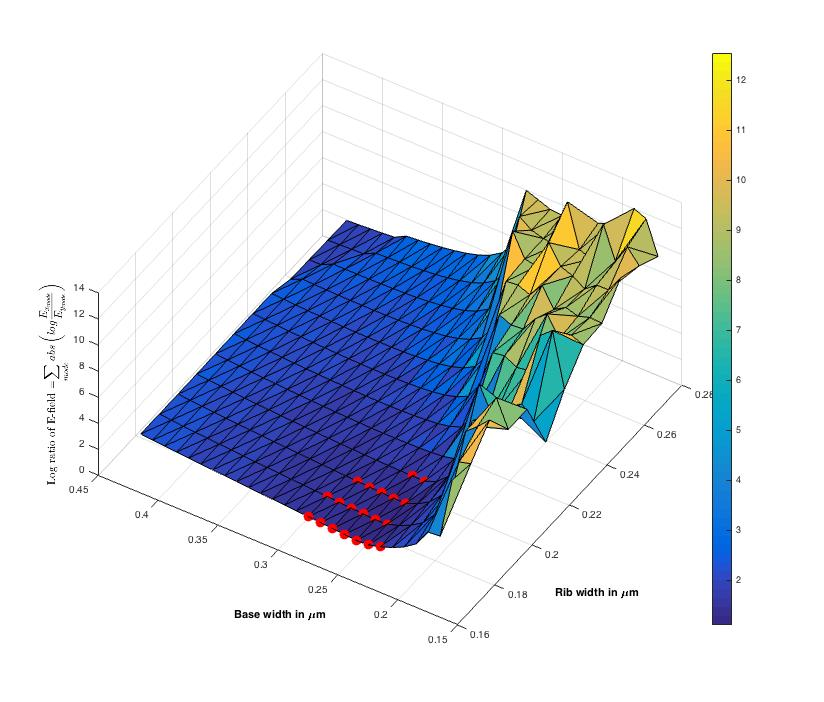
\includegraphics[width=1\textwidth]{3-graph-mode-sum-90nm-slab-height}
	\caption{20 least values, representing the summation of real part of absolute value of the logarithmic ratio of $\chem{E_x}$ and $\chem{E_y}$ fields, plotted against rib and total width in an area chart using MATLAB for Slab height = 90nm}
	\label{fig:3_graph_mode_sum_90nm_slab_height}
\end{figure}

\subsubsection{Representational design based on simulation}			
Based on the simulations performed and the dimensions of the cross-section obtained the tunable \gls{pr} was designed as depicted in Fig. \ref{fig:3_wg_design_1_mems}. However, for quicker simulation purposes the remaining portions of the \gls{mems} waveguide cantilever are not considered in the simulation design.  

\begin{figure}[H] %h
	\centering
	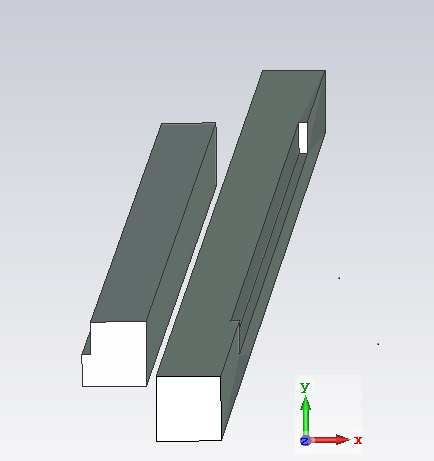
\includegraphics[width=0.75\textwidth]{3-wg-design-1-mems}
	\caption{Design of single-stair waveguide with MEMS tuning waveguide. Stair cross-section dimensions are: $\chem{Rib_{width}}$ = 200nm, $\chem{Rib_{height}}$ = 110nm, $\chem{Slab_{width}}$ = 230nm, $\chem{Slab_{height}}$ = 110nm, and cross-section length = \SI{51}{\micro\meter}, in both the PR waveguide and MEMS waveguide. The output port is along the Z-axis}
	\label{fig:3_wg_design_1_mems}
\end{figure}

\begin{figure}[H] %h
	\centering
	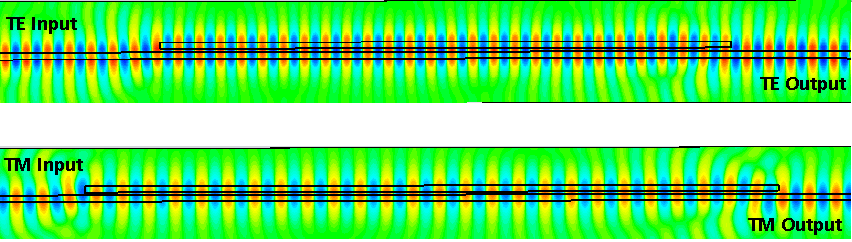
\includegraphics[width=0.75\textwidth]{3-wg-tpr-mems-transmission}
	\caption{Transmission with a \gls{mems} waveguide for \gls{tpr} in Silica cladding}
	\label{fig:3_wg_tpr_mems_transmission}
\end{figure}

\begin{comment}

		\subsection{Design B: Tapered Si waveguide with horizontal gradual asymmetry on SOI with air cladding based on mode evolution}

\subsubsection{Optimized dimensions of bus waveguide}
		
\begin{figure}[H] %h
	\begin{subfigure}[t]{0.45\textwidth}
		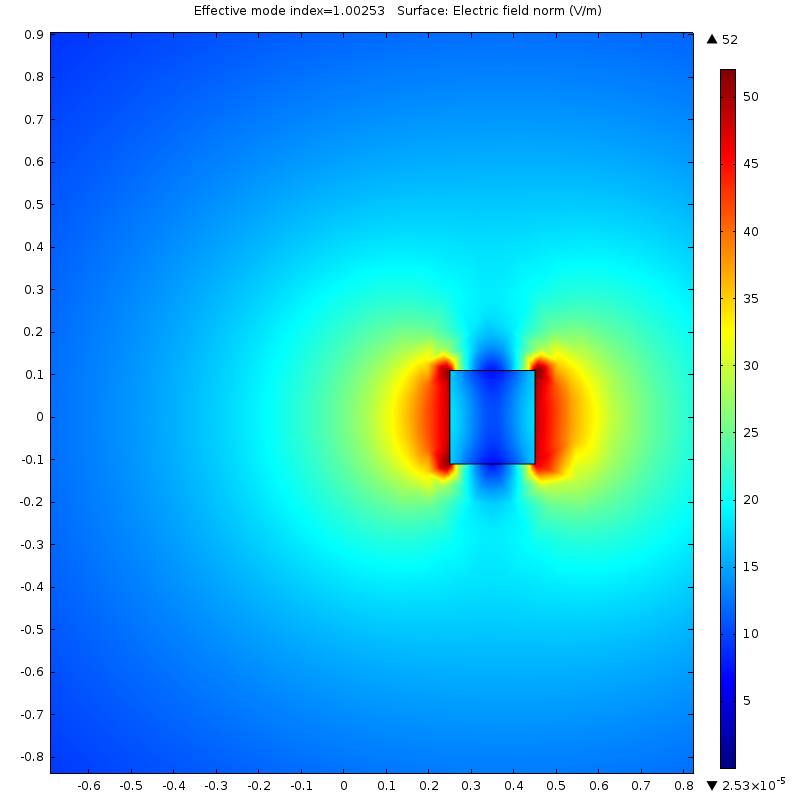
\includegraphics[width=\textwidth]{3-mode1-200-200}
		\caption{\gls{te} mode in the cross-section}
		\label{fig:3_mode1_200_200}
	\end{subfigure}
	\hfill
	\begin{subfigure}[t]{0.45\textwidth}
		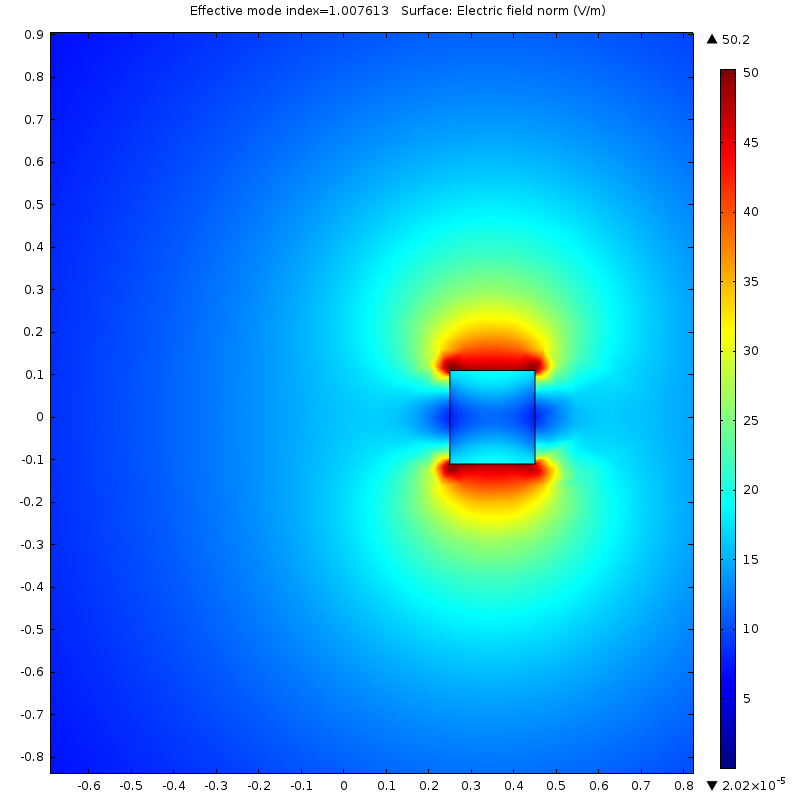
\includegraphics[width=\textwidth]{3-mode2-200-200}
		\caption{\gls{tm} mode in the cross-section}
		\label{fig:3_mode2_200_200}
	\end{subfigure}
	\caption{Hybrid modes in the cross-section with width = 200nm, height = 220nm, obtained using Comsol 2-D simulation}
\end{figure}

\subsubsection{Optimized dimensions of MEMS waveguide}	

\subsubsection{Device tolerance}

\subsubsection{Representational design based on simulation}
\end{comment}

\section{Designing auxiliary components for measurement setup}
To test the \gls{tpr} auxiliary components like grating couplers (\gls{te} \& \gls{tm}), tapers, \gls{pbs} are designed. The gratings are designed in way to couple \gls{te} and \gls{tm}-modes from the LASER to the waveguide taper. The tapers are connected to the \gls{tpr}, to reduce the mode size. Finally, a \gls{pbs} is designed which again decouples the \gls{te} and \gls{tm}-modes to the grating couplers via tapers where a photo-detector measures the intensity of output light. Another approach like butt-coupling can be used. But it is difficult to couple light into narrow waveguides in a low-loss manner as the mode size is bigger.  

\begin{figure}[H] %h
	\centering
	\includegraphics[width=1\textwidth]{3-sys-design}
	\caption{System level block diagram of the fabricated device}
	\label{fig:3_sys_design}
\end{figure}
\noindent In the Fig. \ref{fig:3_sys_design} a high level block diagram of the measurement setup is shown. Whereas, in Fig. \ref{fig:3_tpr_test_setup} top view of the low level system design is shown with gratings, tapers, \gls{tpr}, \gls{tm} coupler and bridges. 
\begin{figure}[H] %h
	\centering
	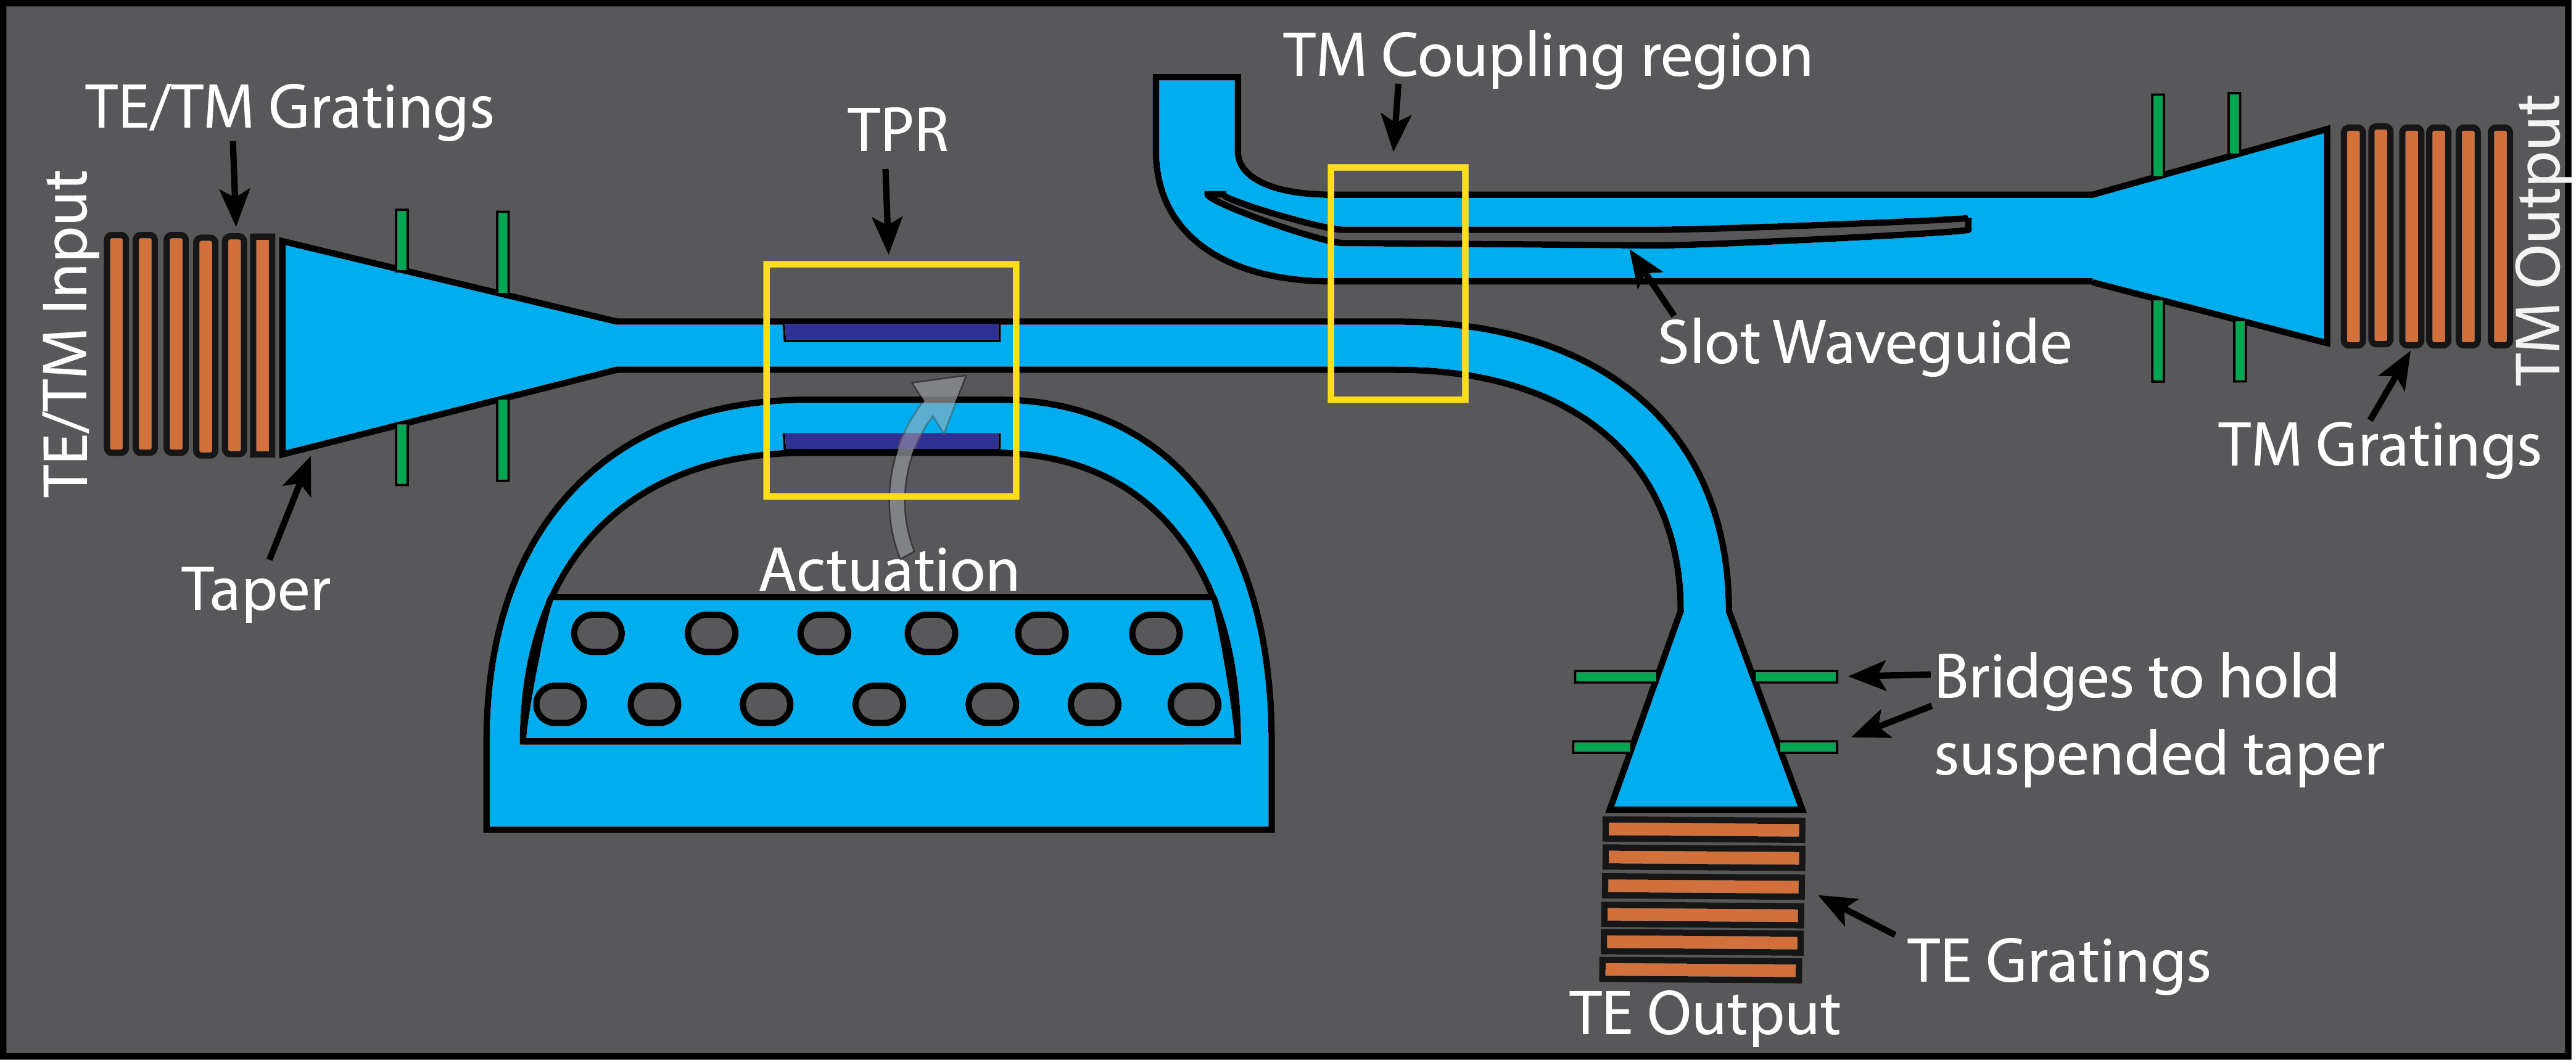
\includegraphics[width=1\textwidth]{3-tpr-test-setup}
	\caption{Top view schematic representation of the measurement setup}
	\label{fig:3_tpr_test_setup}
\end{figure}

\subsection{Grating coupler design}
The high effective index and small mode dimensions of single mode silicon waveguides makes fiber coupling challenging. Waveguide-to-fiber surface grating couplers with fill factor apodization offer low back reflection into the silicon waveguide and a single required lithography step. Using surface grating couplers, the mode matching problem can be solved by expanding the width of the on-chip silicon waveguide, and etching a grating into the expanded section that diffracts light out of plane into a fiber placed normal to the surface. The approach taken increases the coupling efficiency by tailoring the leakage factor of the grating to the mode profile of the fiber. The main benefits of this approach are a low back reflection into the silicon waveguide and high efficiency in the coupling \cite{grating_coupler}. In the design, the gratings used are \SI{1200}{\nano\meter} wide which narrows down to a width of \SI{230}{\nano\meter} in the \gls{pr} section. The approach is shown in Fig. \ref{fig:3_gc_setup}.

\begin{figure}[H] %h
	\begin{subfigure}[t]{0.45\textwidth}
		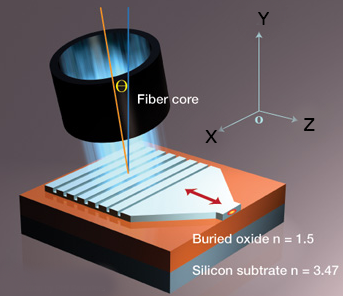
\includegraphics[width=\textwidth]{3-gc-setup}
		\caption{Fiber to waveguide surface coupling using grating coupler}
		\label{fig:3_gc_setup}
	\end{subfigure}
	\hfill
	\begin{subfigure}[t]{0.45\textwidth}
		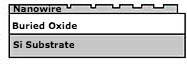
\includegraphics[width=\textwidth]{3-gc-cross-section}
		\caption{Apodized grating coupler cross-section}
		\label{fig:3_gc_cross_section}
	\end{subfigure}
	\caption{Overview of surface coupling from fiber to waveguide using apodized grating coupler with cross-sectional view}
\end{figure}


\subsection{Taper with slab design}
While tapering down to the \gls{tpr} cross-section from the grating coupler cross-section, the $\chem{SiO_{2}}$ underneath is etched away. Hence, to support the structure from the side bridges are drawn which forms a slab like structure at certain cross-sections. These kinds of structures accommodate mode conversions between $TM_0$ and $TE_3$. Also, these bridges can be used in different places in the test structure where support is necessary to hold the waveguide. For example, if the core waveguide width is \SI{700}{\nano\meter} then a total base width (base and slab) of \SI{1500}{\nano\meter} must be avoided for mode conversion reasons. This is simulated using COMSOL and the results are plotted in Fig. \ref{fig:3_slab_modes_700nm}. As, it can be seen that around \SI{1500}{\nano\meter} base width there is a mode conversion between $\chem{TM_0}$ and $\chem{TE_3}$ represented in Fig. \ref{fig:3_te_1500_slab} and Fig. \ref{fig:3_tm_1500_slab}. 
 
 \begin{figure}[H] %h
 	\centering
 	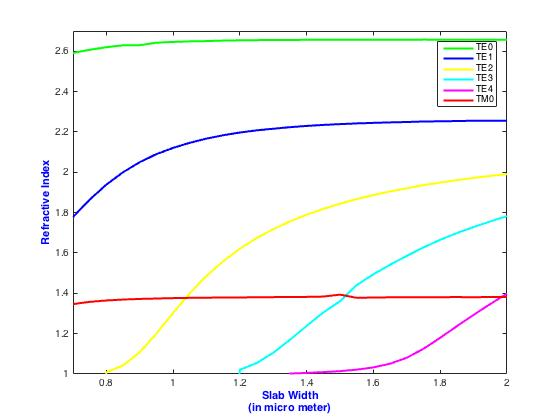
\includegraphics[width=.75\textwidth]{3-slab-modes-700nm}
 	\caption{TE and TM modes at different base widths obtained using COMSOL mode solvers}
 	\label{fig:3_slab_modes_700nm}
 \end{figure}
 
 \begin{figure}[H] %h
 	\begin{subfigure}[t]{0.45\textwidth}
 		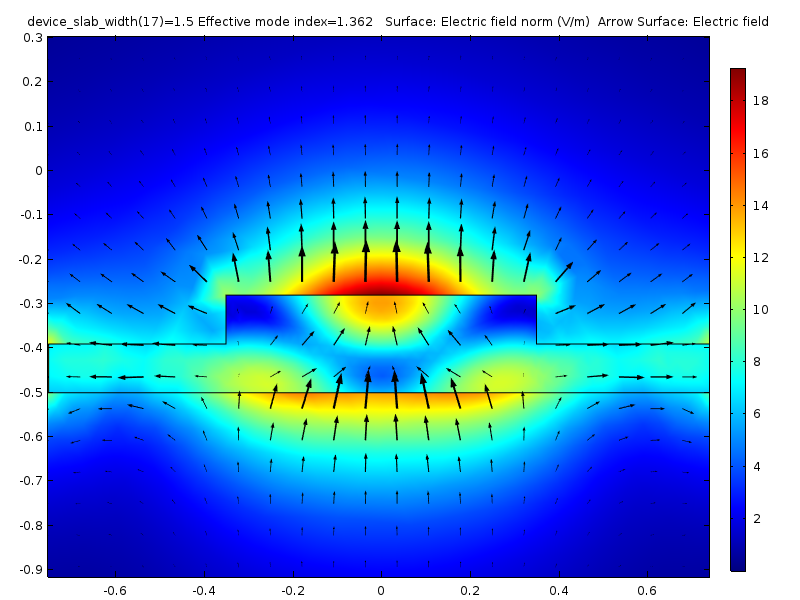
\includegraphics[width=\textwidth]{3-te-1500-slab}
 		\caption{TE mode with $\chem{Base_{width}}$ = 1500nm}
 		\label{fig:3_te_1500_slab}
 	\end{subfigure}
 	\hfill
 	\begin{subfigure}[t]{0.45\textwidth}
 		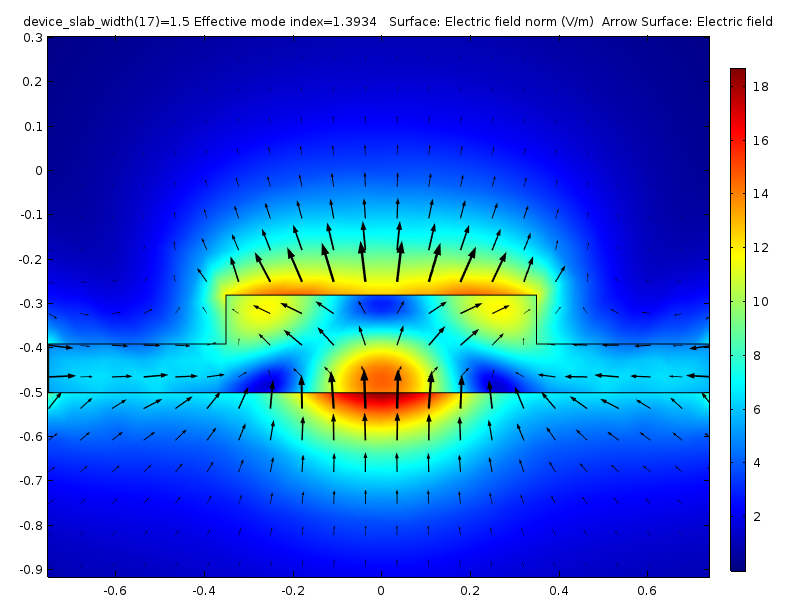
\includegraphics[width=\textwidth]{3-tm-1500-slab}
 		\caption{TM mode with $\chem{Base_{width}}$ = 1500nm}
 		\label{fig:3_tm_1500_slab}
 	\end{subfigure}
 	\caption{Mode conversion in Slab modes at $\chem{Base_{width}}$ = 1500nm, obtained using Comsol 2-D simulation}
 \end{figure}


\subsection{Polarization beam splitter design}
The \gls{pbs} based on an asymmetrical directional coupler by utilizing the evanescent coupling between a strip-nanowire and a nanoslot waveguide \cite{pbs_dai_2011}. First, \gls{ri} is calculated for different core widths with height = 220nm. The results are displayed in Fig. \ref{fig:3_pbs_core_waveguide}.
\begin{figure}[H] %h
	\centering
	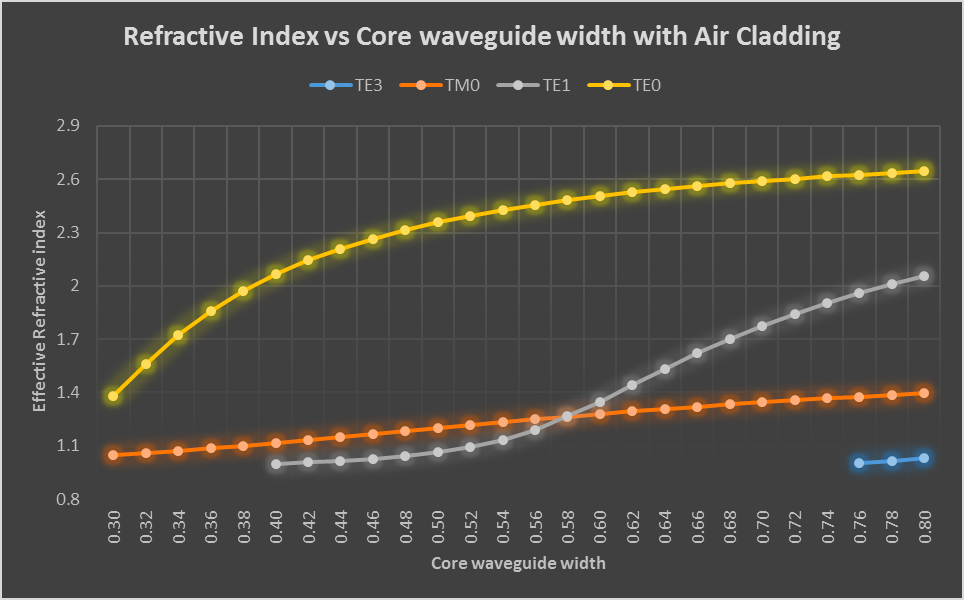
\includegraphics[width=0.75\textwidth]{3-pbs-core_waveguide}
	\caption{\gls{ri} for different dimensions of core waveguide width}
	\label{fig:3_pbs_core_waveguide}
\end{figure}
\noindent Next, the \gls{ri} is calculated for different widths of nanoslot waveguide with a height of 220nm and slot width of 100nm. The gap between the core waveguide and the nanoslot waveguide is 150nm. The results are plotted in Fig. \ref{fig:3_pbs_slot_waveguide}.
\begin{figure}[H] %h
	\centering
	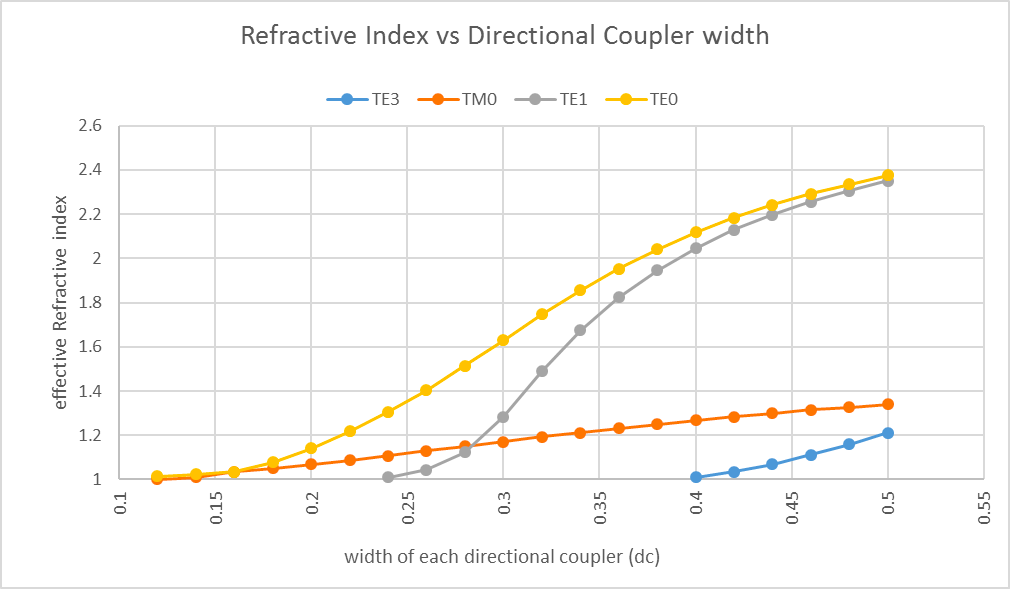
\includegraphics[width=0.75\textwidth]{3-pbs-slot_waveguide}
	\caption{\gls{ri} for different dimensions of slot cross-section}
	\label{fig:3_pbs_slot_waveguide}
\end{figure}
\noindent It can be seen in Fig. \ref{fig:3_pbs_core_waveguide} that the effective index of $TM_0$ at a width of 550nm is 1.20. Whereas, it can be seen in Fig. \ref{fig:3_pbs_slot_waveguide} that the effective index of 1.20 in $TE_1$ is obtained around a width of 330nm for each section of the nanoslot waveguide. Also, the supermodes are checked in the cross-section keeping the strip-nanowire and the nanoslot waveguide to understand the coupled modes shown in Fig. \ref{fig:3_pbs_te_coupling} and Fig. \ref{fig:3_pbs_tm_coupling}.
\begin{figure}[H] %h
	\begin{subfigure}[t]{0.45\textwidth}
		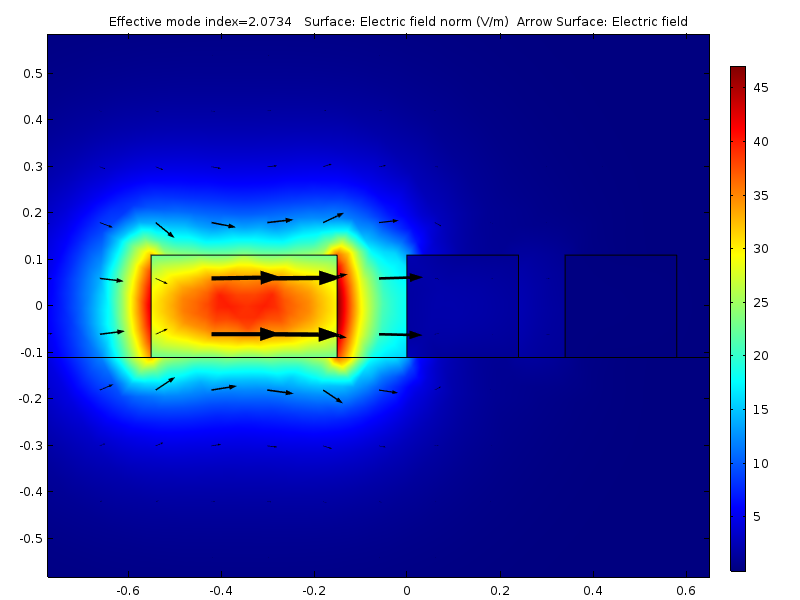
\includegraphics[width=\textwidth]{3-pbs-te-coupling}
		\caption{\gls{te} coupling in the mode coupling cross-section}
		\label{fig:3_pbs_te_coupling}
	\end{subfigure}
	\hfill
	\begin{subfigure}[t]{0.45\textwidth}
		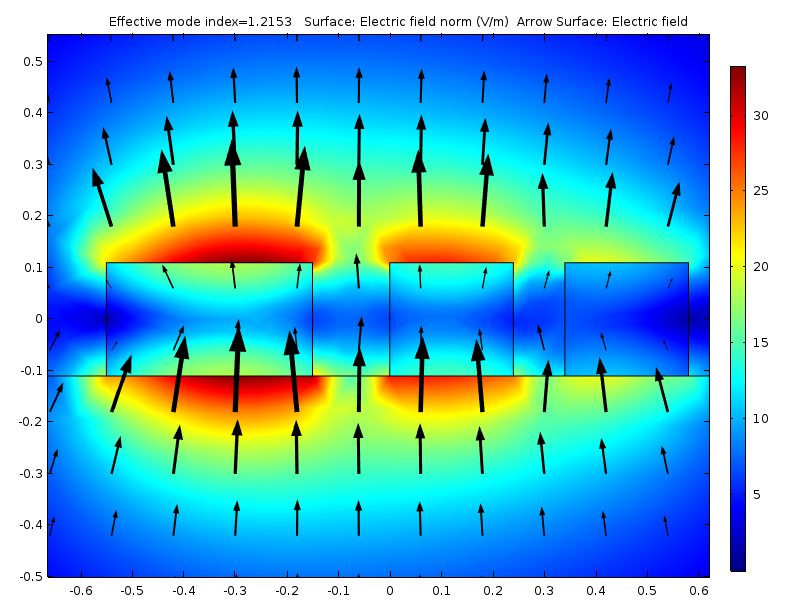
\includegraphics[width=\textwidth]{3-pbs-tm-coupling}
		\caption{\gls{tm} coupling in the mode coupling cross-section}
		\label{fig:3_pbs_tm_coupling}
	\end{subfigure}
	\caption{\gls{te} and \gls{tm} coupling in \gls{pbs} slot waveguide at the mode coupling region}
\end{figure}

\noindent Finally, the designed is simulated in 3-D using CST for checking the transmission with strip-nanowire of width 500nm and nanoslot waveguide of width 330nm each with slot width of 100nm. The coupling length is estimated from \ref{eq:lpi_calc}. As, $n_{TE0}$ = 2.35 and $n_{TM0}$ = 1.20, hence $L_{\pi}$ = \SI{1.4}{\micro\meter}. As seen in Fig. \ref{fig:3_te_coupler}, the TE goes through the without coupling. Whereas, as seen in Fig. \ref{fig:3_tm_coupler}, the TM mode crosses through in the coupling region. As, it can be seen some portion of the TM mode goes through as well. However, the measured \gls{per} is more than 15dB. The purpose of this setup is to make sure that both TE and TM modes can be measured at different ports. In the final design in the measurement setup the nanoslot waveguide is not bend after the coupling region to minimize bents for TM. As TM mode is highly deconfined, bends can cause lossy transmission. Whereas, sine TE mode is confined the strip-nanowire core waveguide is given a sharp bend to minimize coupling beyond the coupling region. 

\begin{figure}[H] %h
	\begin{subfigure}[t]{0.45\textwidth}
		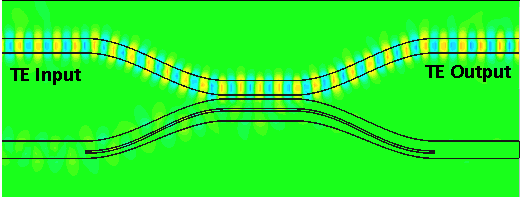
\includegraphics[width=\textwidth]{3-te-coupler}
		\caption{\gls{te} mode through}
		\label{fig:3_te_coupler}
	\end{subfigure}
	\hfill
	\begin{subfigure}[t]{0.45\textwidth}
		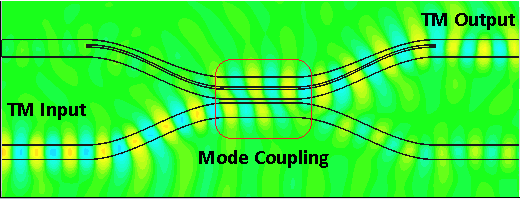
\includegraphics[width=\textwidth]{3-tm-coupler}
		\caption{\gls{tm} mode crossing at the coupling region}
		\label{fig:3_tm_coupler}
	\end{subfigure}
	\caption{\gls{pbs} with \gls{tm} coupling due to mode matching using a slot waveguide}
\end{figure}


\end{document}
